\section{Project Group Room}
\label{sec:projGroupRoomImpl}
In this section the actual implementation of the project group room, its custom blocks, how the context system is used to implement our own context to allow better administration of blocks and capabilities, and the navigation to the users project groups is described.
The section presents how the project groups work from the perspective of the user. 


\subsection{The Page}
\label{sub:page}
The project group page is the virtual meeting place described in \secref{sec:projectgroup}.
We decided to implement the room merely as a container for blocks. 
Alternatively the functionality could be an integrated part of the page, but using blocks gives more flexibility to the users allowing them manage the layout of their own project group room. 
A screenshot of a project group room can be seen in \figref{fig:projectgroupnoedit}. 
In this project group room the blocks of the standard layout are seen.
\begin{figure}[h]
	\centering
		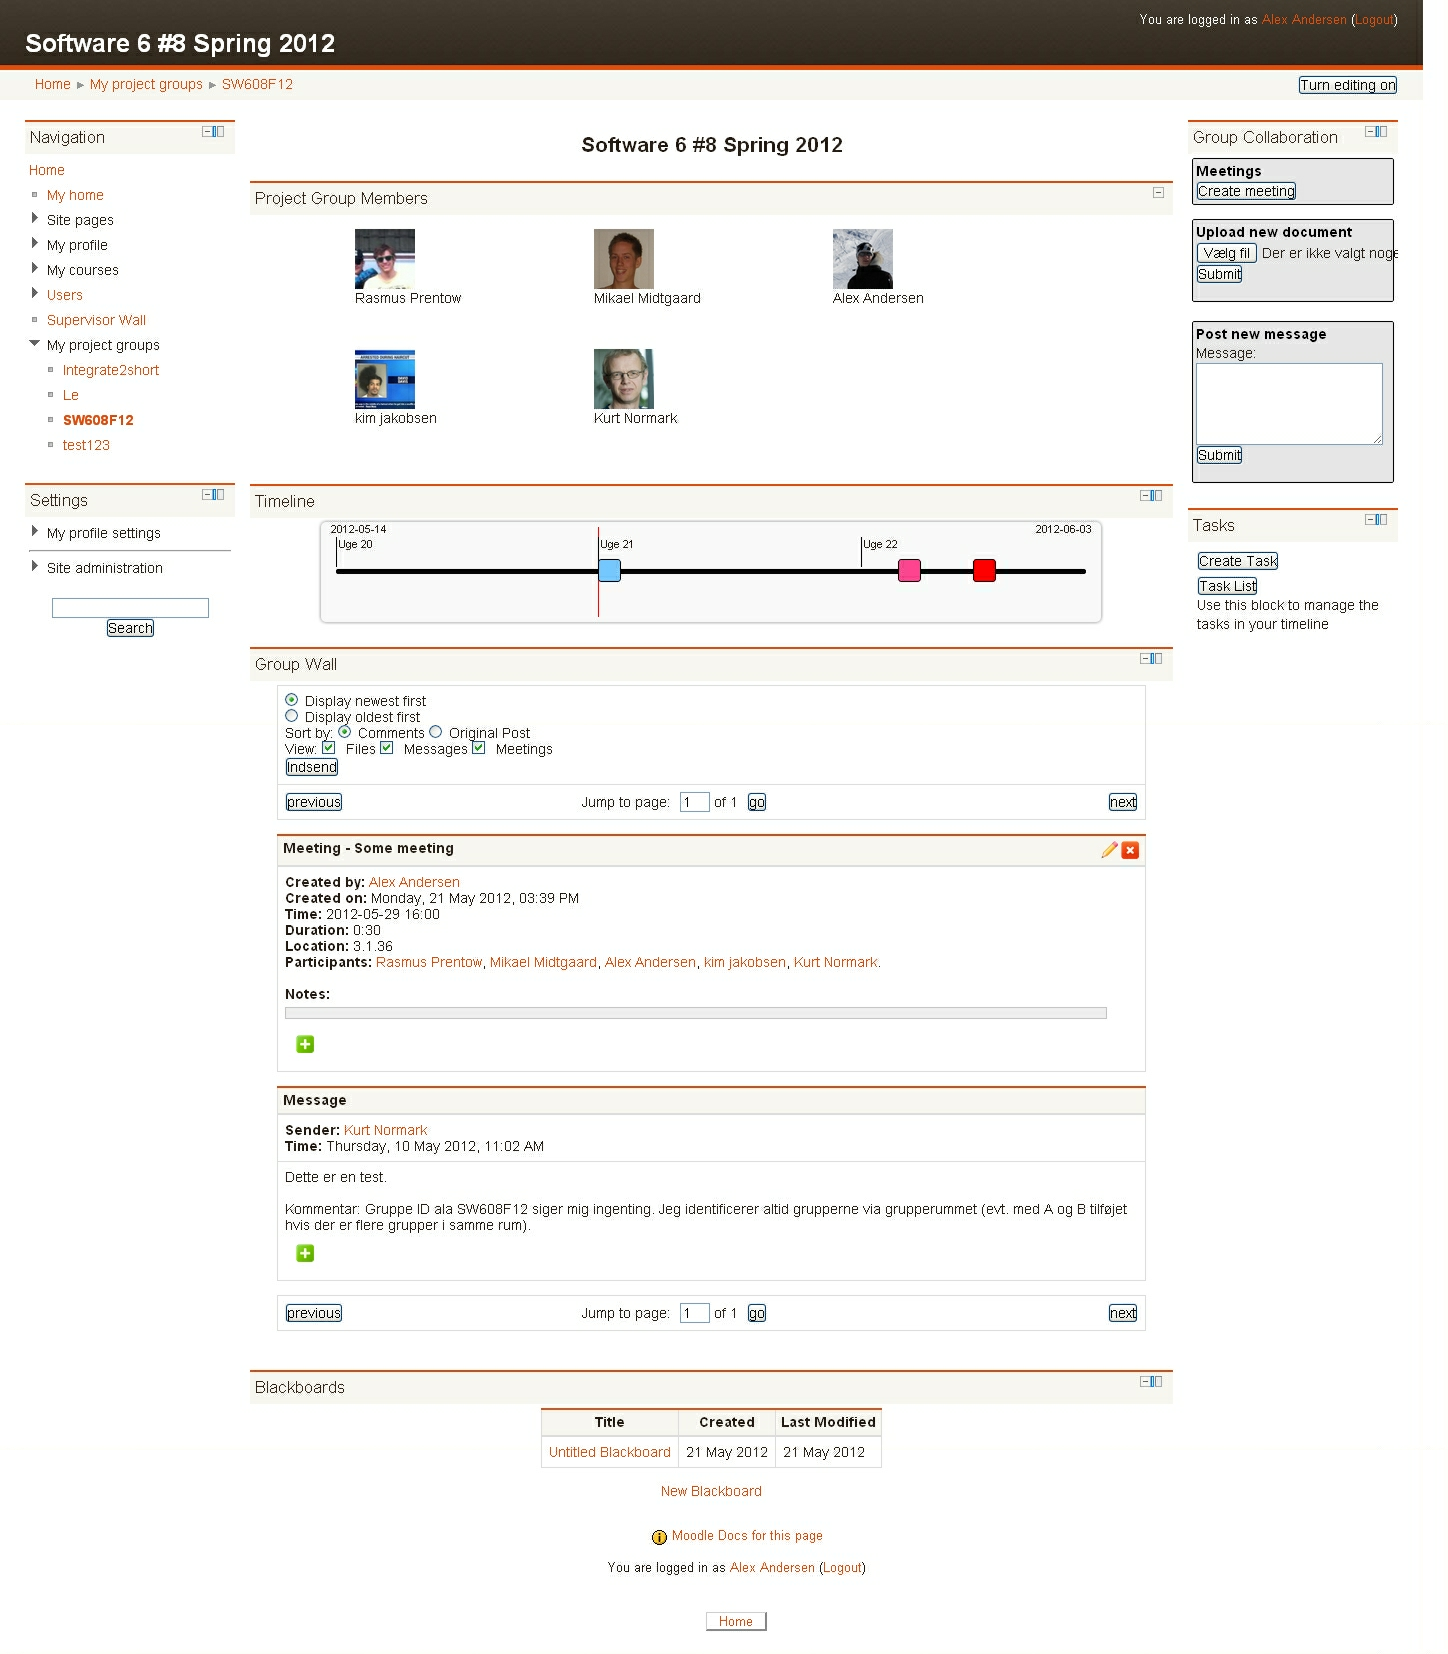
\includegraphics[width=\textwidth]{images/projectgroupnoedit.png}
	\morscaption{The project group room}
	\label{fig:projectgroupnoedit}
\end{figure}

The project group room consist of three columns. 
The left column is the standard navigation menu in Moodle. 
We do not want anything to be added to this column to ensure that the page seem familiar to the user.
The center and right columns both contain blocks.
The various blocks presented on the project groups page are described in \secref{sec:implprojectgroupblocks}. 
If a user wants to edit the block layout for the project group room he can press the ``Turn editing on'' button. 
This will add edit and move buttons to each block. 
A new block is added in editing mode to allow for adding new blocks. 
If a user edits the page, the change can be seen by all group members. 
The page in edit mode can be seen in figure \figref{fig:projectgroupwithedit}.

\begin{figure}[h]
	\centering
		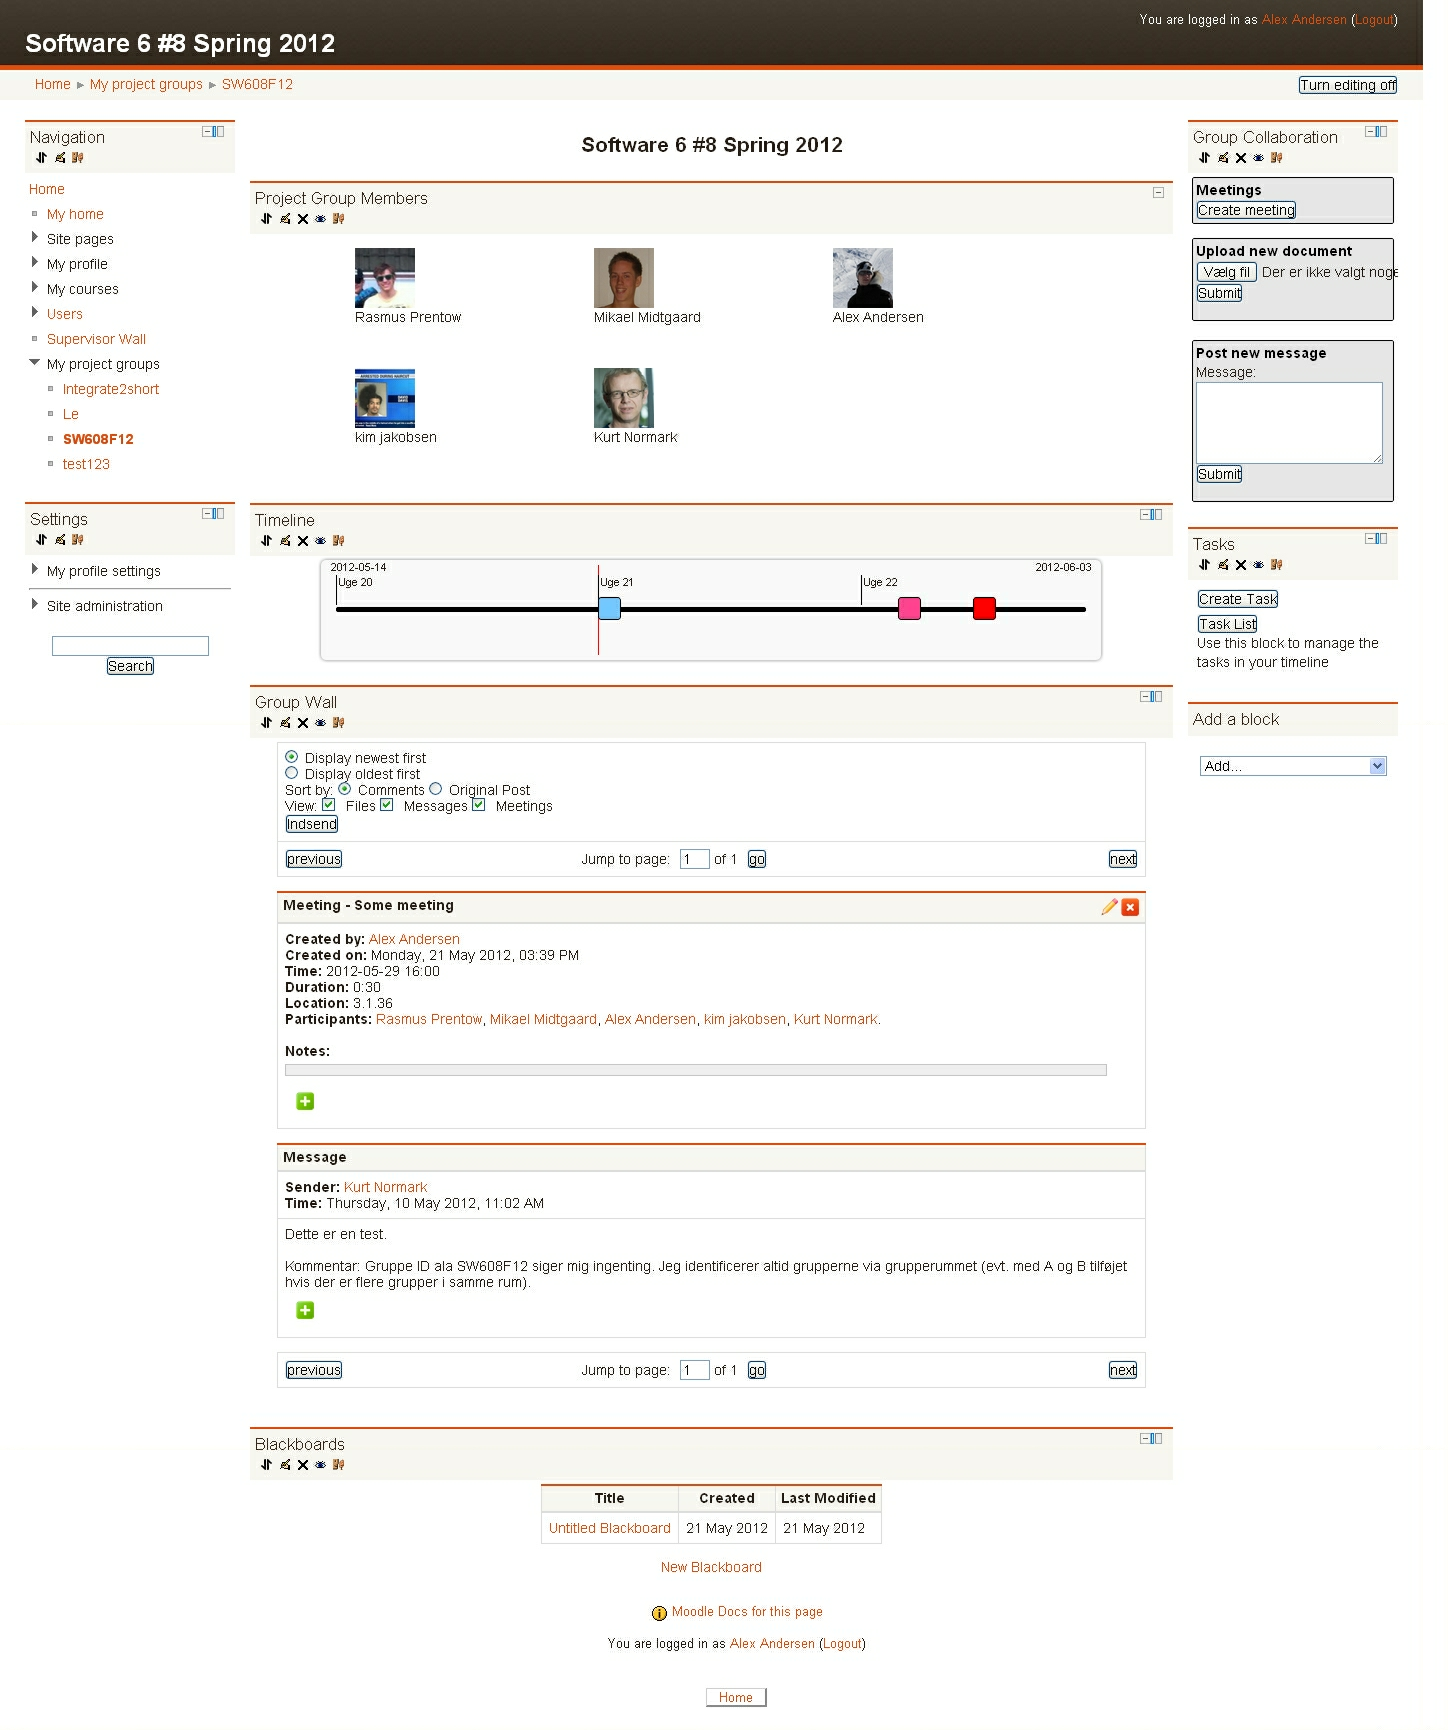
\includegraphics[width=\textwidth]{images/projectgroupwithedit.png}
	\morscaption{The project group room with editing turned on}
	\label{fig:projectgroupwithedit}
\end{figure}


The task of securing that only members of the project group can edit and view are maintained by the project group room and is described in \secref{sec:projectgrouproommanagerights}. 



\FloatBarrier
\subsection{Ensuring Permissions}
\label{sec:projectgrouproommanagerights}
Permissions can generally be divided in two types; read and write. 
Read permissions gives you the ability to view the content of the project group room while write lets you change the content. 
If a user has write permission he must also have read permissions. 
Otherwise he cannot see the page he attempts to edit. 
To ensure the user attempting to enter a project group room has permission to enter the function \fu{has\_projectgroup\_read\_permission} is used. 
It checks if the user is an administrator or is a member of the group. 
The administrator check is necessary since administrators should be able to see the group even if they are not members of the group. 

The function  \fu{has\_projectgroup\_write\_permission} which checks that the user has write permissions uses the read permissions function to check that the user can read.
If he cannot read he should not be able to edit. 
In the current implementation the write permissions function does not make extra checks to permissions since the permission levels for read and write are equivalent.
Making both function gives the ability to later change this.
An example could be if the potential users requires that their supervisor should only have read permissions. 
Then the change will be in one place only. 

\subsection{Blocks}
\label{sec:implprojectgroupblocks}
When a new project group is created the default blocks are added to the page. 
The default blocks are specified in the a config file and the content can be seen in \coderef{moodledaultblock}


\begin{lstlisting}[style=phpCode, caption=\myCaption{The default block configuration}, label=moodledaultblock]
<?php
	/**
	* Example usage:
	* "left1,left2:center1:right1"
	* Will add two items to the left, one in the middle, and one to the right
	*/
	$format['defaultprojectgroupblocks'] = ':projectgroup_members,timeline,groupwall,blackboard:upload,tasks';
\end{lstlisting}\begin{comment}$\end{comment}
The syntax for the format is $left:middle:right$. 
Left, middle, and right represent the three columns in the project group room. 
The blocks: Timeline, groupwall, blackboard, upload, and tasks is created by our peer-groups while the block named projectgroup\_members is created by us. 
The projectgroup\_members block shows the name and pictures of the project group members. 

	
	


\subsection{Overwrite Context}
In \secref{sub:contextsystem}  the context system of Moodle is described.
In this section the creation of a custom context is described. 

To be able to define capabilities for the project groups and have different blocks for different project group we need our own context.
We will create our own context level and class.
We call the context \cl{context\_projectgroup}. 

Moodle does not support extension of contexts through one of the more than 30 different plugin types available \cite{plugin}. 
There two parts of the problem, the first is to create a new context and the second is to load it properly. 
We create a new context by making a new class which is very similar to \cl{context\_course} class and by defining the context level of project groups as a constant. 
The class header and the constant definition can be seen in \coderef{codeprojectgroupcontext}. 
The constant is set to 55 and is chosen because that context level is unused and it is close to the course context level. 
We regard the project group contexts to be at the same level as course contexts. 
However, project groups does not have categories like courses does.

\begin{lstlisting}[style=phpCode, caption=\myCaption{The context\_projectgroup class header and constant definition}, label=codeprojectgroupcontext]
define ('CONTEXT_PROJECTGROUP',55);
class context_projectgroup extends context {
...
\end{lstlisting}

When a context is loaded in a Moodle page it is instantiated by \fu{get\_context\_instance}, which takes a context level and an instance id. 
The instance id can be a course id or similar depending on the context level -- in our case it is a project group id. 
This function calls a static method in the \cl{context\_helper} class which uses a private array to translate the context level into a class name.
The overall system definition in \chapref{chap:systemDef} retain us from changing the core code of Moodle. 
If this constraint were not enforced the array could simply be extended directly in the code.  
Since the array used is private we can not extend the context system by overriding the \cl{context\_helper} class. 
The newly created context is only used in pages created in this project and we can therefore create our own version of \fu{get\_context\_instance}. 
The new function can be seen in \coderef{codeprojectgroupcontextinstance}.
\begin{lstlisting}[style=phpCode, caption=\myCaption{The function to get projectgroup context}, label=codeprojectgroupcontextinstance]
function get_projectgroup_context_instance( $instance = 0, $strictness = IGNORE_MISSING) 
{ 
    return context_projectgroup::instance($instance, $strictness);
}
\end{lstlisting}
The \vari{instance} variable denotes a project group id.
The \vari{strictness} variable 

With the new context and the function to instantiate it we can now make per project group permissions and add blocks to specific project group pages. 



\subsection{Navigation}
%In \secref{sub:designprojectgroupnavigation} the navigation to project groups is described and in this section the actual implantation of the navigation described. 
In \secref{sec:requirements} we have a requirement called \req{Navigate to Project Groups} which states that a user should be able to find the project group(s) that he is a member of.
This implementation that satisfies this requirement is presented here.
Since we implement the project group room as a local plugin we can use a build-in functionality of \moodle{} to extend the navigation block~\cite{moodleextendnavigationblock}.
The navigation menu can be seen in \figref{fig:moodlenavigationblock}.
The extended part is highlighted by the rectangle. 

\begin{figure}
	\centering
		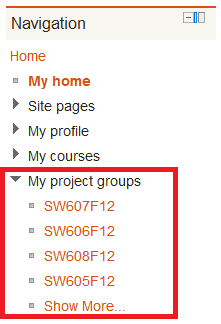
\includegraphics[scale=0.7]{images/moodlenavigationblock.png}
		\morscaption{\moodle{} navigation bar. The highlighted box shows our extension with a list of project groups, which the currently logged in user is a member of}
	\label{fig:moodlenavigationblock}
\end{figure}

The code to add project groups to the navigation can be seen in \coderef{src:moodlecodeextendingnavigation}.
The currently logged in user is accessed to get the project groups that he is a member of.
The code checks if something should be displayed at all and then run a loop to print out the link to each group. 
If more than four project groups is associate with the given user a link to show more is added and no more links are generated.


\begin{lstlisting}[style=phpCode, caption=\myCaption{The code for extending the navigation}, label=src:moodlecodeextendingnavigation]
function projectgroup_extends_navigation(global_navigation $navigation) 
{
	global $USER;
	$number_of_groups = 4;
	
		...
	
	$groups = get_groups_of_user($USER->id);
	if(sizeof($groups) > 0)
	{
		$type = navigation_node::TYPE_CUSTOM;
		$my_projectgroup_navigation = $navigation->add(get_string('myprojectgroup','local_projectgroup'),null,$type,null,'myprojectgroup');
		$count = 0;
		foreach ($groups as $group_id) 
		{
			$count++;
			if($count > $number_of_groups ){
				$my_projectgroup_navigation->add('Show More...', 
					new moodle_url('/local/projectgroup/usergroups.php',
					array('id'=>$USER->id, 'sesskey'=>sesskey())),
					$type,null,'show_more');
				break;
			}
			$group = get_projectgroup($group_id);
			$my_projectgroup_navigation->add($group->shortname, new moodle_url('/local/projectgroup/index.php', array('id'=>$group_id, 'sesskey'=>sesskey())),$type,null,$group->id);
			
		}
	}
}
\end{lstlisting}




















